\documentclass[alternative-exam.tex]{subfiles}
\begin{document}

\chapter{Tussentijdse Toets}

\section{Vraag}
Professor Veys geeft een tussentijdse toets voor Lineaire Algebra in week 9 van het eerste semester.
Hij wil rekening houden met de voorkeuren van alle richtingen die deze toets krijgen. De jaarverantwoordlijken van wiskunde, fysica en informatica geven hun voorkeuren door. De voorkeuren zien er als volgt uit.\\\\
De wiskundigen gaan graag naar de winabar en willen daarom de toets liefst niet op donderdag. De fysici hebben op dinsdag een andere tussentijdse toets en zouden het liefst minstens één dag na die toets geen toets hebben, zodat ze tijd hebben om te studeren. De informatici willen de toets liefst niet op maandag, omdat er dan een deelexamen van SOCS plaatsvindt.\\\\
Professor Veys zet het liefst de toets voor de informatici als eerst, omdat die verbetering het langst duurt. Bovendien wil hij niet dat de drie toetsen op dezelfde dag vallen maar hij wil ook niet er dagen tussen de toetsen zijn. Hij wil dus de drie toetsen op drie opeenvolgende dagen zetten.\\\\
Hoe plant Professor Veys best de tussentijdse toets voor de drie richtingen? (Hij wil alle toelaatbare oplossingen)

\section{Modeloplossing}
We lossen dit probleem om met constraint processing technieken. We zullen de beperkingen formeel defini\"eren, en er een constraint processing oplossingsmethode op uitvoeren.
\subsection{Formele formulering}
\begin{figure}[H]
\centering
\caption{Waarden voor dagen}
\label{waarde_dagen}
\begin{tabular}{| c | c | }
\hline
dag & waarde\\
\hline
maandag & 1\\
dinsdag & 2\\
woensdag & 3\\
donderdag & 4\\
vrijdag & 5\\
\hline
\end{tabular}
\end{figure}
We kiezen drie variabelen. Noem $z_f$, $z_w$, $z_i$ respectievelijk de dag waarop fysica, wiskunde en informatica de toets krijgt. Om de beperkingen makkelijk op te schrijven wijzen we aan elke dag van maandag tot vrijdag in week 9 (de dagen dat er een toets gegeven kan worden) een getal toe zoals beschreven in figuur \ref{waarde_dagen}.
Nu kunnen we de constraints formuleren volgens deze waarden.

\subsubsection{Unaire beperkingen}
De unaire beperkingen krijgen we toevallig allemaal van de richtingen.\\
De Wiskundigen willen hun toets niet op donderdag.
\[
z_w \neq 4
\]
De fysici willen hun toets ten vroegste twee dagen na dinsdag.
\[
z_f > 3
\]
Tenslotte willen de informatici de toets niet op maandag.
\[
z_i \neq 1
\]
We kunnen nu de unaire beperkingen als volgt samenvatten.
\[
\left\lbrace
\begin{array}{c c c}
c(z_w) & \leftrightarrow & z_w \neq 4\\
c(z_f) & \leftrightarrow & z_f > 3\\
c(z_i) & \leftrightarrow & z_i \neq 1\\
\end{array}
\right.
\]
\subsubsection{Binaire beperkingen}
Professor Veys zorgt voor de binaire constraints. Hij wil de toets als eerst aan de informatici geven.
\[
z_i < z_w,\ z_i < z_f
\]
Tenslotte wil hij dat elke toets op een andere dag valt en dat er geen dagen tussen twee toetsen zitten.
\[
z_i \neq z_w,\ z_i \neq z_f,\ z_w \neq z_f
\]
\[
|z_i - z_w| \le 2,\ |z_w - z_f| \le 2,\ |z_i - z_f| \le 2
\]
De binaire beperkingen vatten we nu als volgt samen
\[
\left\lbrace
\begin{array}{c l l c c c c}
c(z_w, z_f) & \leftrightarrow && & z_w \neq z_f &\wedge& |z_w - z_f| \le 2\\
c(z_f, z_i) & \leftrightarrow & z_i < z_f &\wedge& z_i \neq z_f &\wedge& |z_i - z_f| \le 2\\
c(z_i, z_w) & \leftrightarrow & z_i < z_w &\wedge& z_i \neq z_w &\wedge& |z_i - z_w| \le 2\\
\end{array}
\right.
\]

\subsection{Domein}
Het domein van de variabelen bespreek ik als laatst omdat dit nog verkleind kan worden als we rekening houden met node consistentie.
Aanvankelijk hebben alle variabelen het domein $d_\bullet = \{1,2,3,4,5\}$. Door rekening te houden met de unaire beperkingen van variabelen kunnen we hun domein kleiner maken.
\[
\left\lbrace
\begin{array}{r l}
d_{z_w}' &= \{1,2,3,5\}\\
d_{z_f}' &= \{4,5\}\\
d_{z_i}' &= \{2,3,4,5\}\\
\end{array}
\right.
\]

\subsection{Constrant network}
\begin{figure}[H]
\caption{Constraint Network}
\label{fig:fourTeachersConstraintNetwork}
\centering
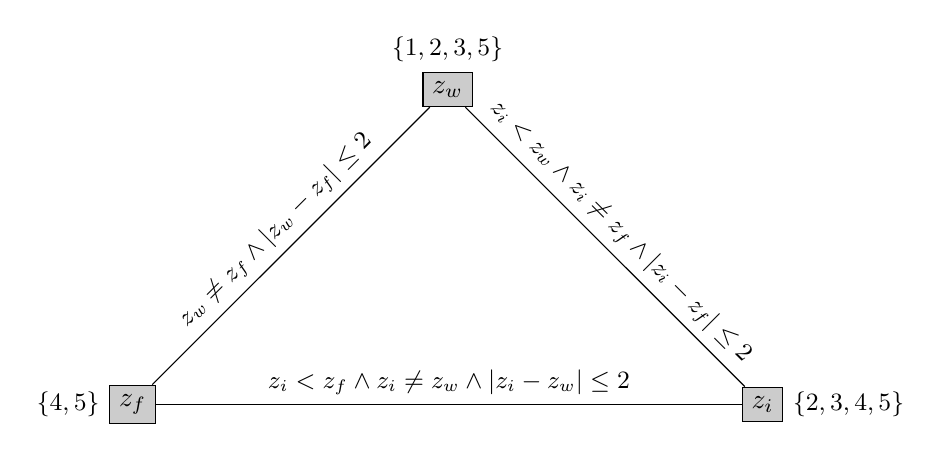
\begin{tikzpicture}[vari/.style={fill=black!20,rectangle,draw=black}]
\def\dx{4};
\def\dy{4};
\def\r{0.125};
\node[vari] (A) at (0,\dy) {$z_w$};
\node[vari] (B) at (-\dx,0) {$z_f$};
\node[vari] (C) at (\dx,0) {$z_i$};

\node[anchor=south] (DA) at (A.north) {\small{$\left\{1,2,3,5\right\}$}};
\node[anchor=east] (DB) at (B.west) {\small{$\left\{4,5\right\}$}};
\node[anchor=west] (DC) at (C.east) {\small{$\left\{2,3,4,5\right\}$}};

\draw (A) to node[midway,sloped,above]{\small{$z_w \neq z_f \wedge |z_w - z_f| \le 2$}} (B);
\draw (A) to node[midway,sloped,above]{\small{$z_i < z_w \wedge z_i \neq z_f \wedge |z_i - z_f| \le 2$}} (C);
\draw (B) to node[midway,sloped,above]{\small{$z_i < z_f \wedge z_i \neq z_w \wedge |z_i - z_w| \le 2$}} (C);
\end{tikzpicture}
\end{figure}
Als samenvatting van heel het probleem kunnen we het zogenaamde constraint network opstellen. Zie figuur \ref{fig:fourTeachersConstraintNetwork}.

\subsection{Uitwerking van forward checking}
We zullen nu de methode 'forward checking' toepassen op dit probleem. Omwille van effici\"entie zullen we een zogenaamde dynamic search rearrangement techniek toepassen. We zullen op elk niveau de waarde kiezen met het kleinste overgebleven domein kiezen om een waarde aan toe te kennen.
Doordat we dynamic search rearrangement gebruiken is de uitwerking van deze oplossing geen grote opdracht nu alle constraints zijn geformuleerd.\\\\
We beginnen bij $z_f$ want deze variabele heeft het kleinste domein, namelijk $\{4,5\}$. We hebben in onze dynamic search rearrangement regels niets gezegd over de volgorde waarin we de elementen van het domein overlopen. Bijgevolg kiezen we het kleinste element eerst.\\\\
We stellen nu $z_f$ gelijk aan $4$ en bekijken alle constraints die iets met $z_f$ te maken. Dit zijn $c(z_w,z_f)$ en $c(z_f,z_i)$. Wanneer we $c(z_w,z_f)$ nakijken, zien we dat in het domein van $z_w$ $1$ wegvalt zodat $\{2,3,5\}$ het nieuwe domein van $z_w$ is. We kijken nu $c(z_w,z_f)$ na en verwijderen $4$ en $5$. Het nieuwe domein van $i$ is nu $\{2,3\}$.\\
$z_i$ is nu de variabele met het kleinste domein. We stellen $i$ gelijk aan $2$. We zien dat $c(z_f,z_i)$ nog steeds geldt. We kijken $c(z_i,z_w)$ nog na en verwijderen daarom $2$ en $5$ ook uit het domein van $z_w$.\\ Het overblijfsel van het domein van $z_w$ is nu $\{3\}$. We stellen $z_w$ gelijk aan $3$ en kijken $x(z_w,z_f)$ en $c(z_i,z_w)$ na. We zien dat beide beperkingen van $z_w$ nog gelden dus de gevonden waarden van de variabelen vormen een oplossing.\\We zijn echter nog niet klaar. Professor Veys wil alle mogelijke oplossingen, dus we moeten nog terug gaan naar v\'o\'or we $2$ aan $z_i$ toekenden. We kennen u $3$ aan $z_i$ toe. We zien dat de beperking tussen $z_f$ en $z_i$ nog steeds geldt. De beperking tussen $z_w$ en $z_i$ zorgt ervoor dat we $2$ en $3$ uit het domein van $z_w$ verwijderen. Tenslotte moeten we nog nakijken dat het overblijvende element in het domein van $z_w$ voldoet aan de beperkingen van $z_w$.
Kennen we $5$ aan $z_w$ toe dan is het makkelijk te zien dat $z_w$ aan $c(z_w,z_f)$ en $c(z_i,z_w)$ voldoet.\\\\
Nu moeten we nog terug gaan naar v\'o\'or we $4$ aan $z_f$ toekenden. De andere waarde die we kunnen toekennen aan $z_f$ is $5$. We doen dit en kijken de beperkingen van $z_f$ na. Uit het domein van $z_w$ verwijderen we $1$, $2$ en $5$ zodat er $\{3\}$ overblijft. Uit het domein van $z_i$ verwijderen we alles, omdat er geen enkele waarde is uit dat domein dat aan de beperkingen tussen $z_f$ en $z_i$ kan voldoen. Omdat het domein van $z_i$ leef wordt is er geen oplossing mogelijk wanneer $f=5$.\\\\
We hebben nu alle oplossingen gevonden.
\[
\left\lbrace
\begin{array}{c c c}
f=4,& w=3,& i=2\\
f=4,& w=2,& i=3\\
\end{array}
\right.
\] 
Deze uitwerking wordt ook nog een beschreven in figuur <TODO VOEG FIGUUR TOE>
\begin{figure}
[p]
\centering
\caption{Uitwerking}
\label{uitwerking}
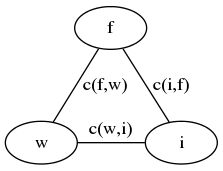
\includegraphics[scale=0.5]{resources/graphs/uitwerking.png}
\end{figure}



\end{document}